%%%%%%%%%%%%%%%%%%%%%%%%%%%%%%%%%%%%%%%%%%%%%%%%%%%%%%%%%%%%%%%%%%%%%%%%%%%%%%%%%%%%%%%%%%%%%%%%%%%%%%%%%%%%%%%%%%%%%%%%%%%%%%%%%%%%%%%%%%%%%
% Latex Template für Zusammenfassungen
% Robin Frauenfelder - September 2018
%%%%%%%%%%%%%%%%%%%%%%%%%%%%%%%%%%%%%%%%%%%%%%%%%%%%%%%%%%%%%%%%%%%%%%%%%%%%%%%%%%%%%%%%%%%%%%%%%%%%%%%%%%%%%%%%%%%%%%%%%%%%%%%%%%%%%%%%%%%%%


\pdfminorversion=6
\documentclass[8pt, a4paper, landscape, xcolor=dvipsnames]{extarticle}
\pagestyle{empty} % Keine Seitennummern

% Verwendete Pakete
    \usepackage{chemfig}
	\usepackage[utf8]{inputenc}
	\usepackage[top=0.7cm, bottom=0.9cm, left=0.65 cm, right=0.65 cm, ]{geometry}
	\usepackage{amsmath}
	\usepackage{amsfonts}
	\usepackage{lmodern}
	\usepackage{graphicx}
	\setlength{\parindent}{0pt}
	\usepackage[normalem]{ulem}
	\usepackage{enumitem}
	\usepackage{mathabx}
	\usepackage{colortbl}
	\usepackage[ngerman]{babel}
	\usepackage{mathtools}
	\usepackage{wallpaper}
	\usepackage{changepage}
	\usepackage{tikz}
	\usepackage{tabularx}
	\usepackage{tcolorbox}
	\usepackage{lipsum}
	\usepackage{multicol}
	\usepackage{letltxmacro}
	\usepackage{tabularx}
	\usepackage{chemformula}
	\usepackage[version=4]{mhchem}
	\usepackage[x-4]{pdfx}
	%\usepackage[dvipsnames]{xcolor}


	\definecolor{Spezi1}{HTML}{512D6D}%lila
	\definecolor{Spezi2}{HTML}{ED680B}%Orange	
	\definecolor{Spezi3}{HTML}{FBB900}%Gelb


	%\definecolor{Spezi1}{HTML}{009EE3}%cyan
	%\definecolor{Spezi2}{HTML}{E5007D}%Orange	
	%\definecolor{Spezi3}{HTML}{FFED00}%Gelb
	

% Spalteneinstellungen

	\setlength\columnsep{3mm}
	\setlength{\columnseprule}{0pt}
	
	
	\setlength{\tabcolsep}{12pt} % Default value: 6pt
    \renewcommand{\arraystretch}{1.8}
            
    % Horizontale Punkte
    \LetLtxMacro\orgddots\ddots
	\DeclareRobustCommand\vdots{%
	  \mathpalette\@vdots{}%
	}
	
	\DeclareRobustCommand\ddots{%
		\mathinner{%
		   \mathpalette\@ddots{}%
		   \mkern\thinmuskip
		}%
	}

	\makeatother
	
	% Schriftart
	\renewcommand{\familydefault}{\sfdefault}
	\newcommand{\cb}{\vfill\null\columnbreak}
	% Dokument-Info Block	

	\newcommand{\DocumentInfo}[1]{
	\begin{tcolorbox}[
		arc=0mm,
		colback=Spezi1,
		colframe=white,
		bottomrule = 0 mm,
		toprule = 0 mm,
		leftrule = 0 mm,
		rightrule = 0 mm,
		valign=center,
		left=0.5mm,
		top= 0.3 mm,
		bottom= 0.3 mm,
		fontupper=\color{white},
		before skip = 0mm,
		leftright skip = -0.5mm,
		after skip = 0 mm]
		\large
	\textbf{#1}	
	\end{tcolorbox}
	}
	
	% Überschrift
	\renewcommand{\section}[1]{
	\begin{tcolorbox}[
			arc=0mm,
			colback=Spezi2,
			colframe=white,
			bottomrule = 0 mm,
			toprule = 0 mm,
			leftrule = 0 mm,
			rightrule = 0 mm,
			valign=center,
			left=0.5mm,
			top= 0.3 mm,
			bottom= 0.3 mm,
			fontupper=\color{white},
			before skip = 0mm,
			leftright skip = -0.5mm,
			after skip = 0 mm]

		\textbf{#1}
	\end{tcolorbox}
	}
		
	
	% Abschnitt	
	\renewcommand{\subsection}[2]{
	\begin{tcolorbox}[
			arc=0mm,
			colback=Spezi3,
			colframe=white,
			bottomrule = 0 mm,
			toprule = 0 mm,
			leftrule = 0 mm,
			rightrule = 0 mm,
			valign=center,
			left=0.5mm,
			top=0.1mm,
			bottom=0.1mm,
			before skip = 0mm,
			leftright skip = -0.5mm,
			after skip = 1.4 mm]
		\small \textbf{#1}
	\end{tcolorbox}
	
	\begin{adjustwidth}{0.5mm}{1mm}
		\footnotesize
		#2
		\vspace{0.5mm}
	\end{adjustwidth}
	}
	
	% Weisser Balken zwischen Abschnitten
	\newcommand{\WhiteSpace}[0]{
	\begin{tcolorbox}[
			arc=0mm,
			colback=white,
			colframe=white,
			bottomrule = 0 mm,
			toprule = 0 mm,
			leftrule = 0 mm,
			rightrule = 0 mm,
			valign=center,
			left=0.5mm,
			top= -0.4 mm,
			bottom= -0.4 mm,
			fontupper=\color{white},
			before skip = 0mm,
			leftright skip = -0.5mm,
			after skip = 0 mm]
	\end{tcolorbox}
	}
	
% Hintergrundbild (graue Spalten)

	\CenterWallPaper{1}{Setup/BackgroundLinien.pdf}

% TabularX Zeug (Paket für Tabellen)

	\newcolumntype{C}[1]{>{\centering\arraybackslash}p{#1}}

% TikZ Zeug (Paket für Vektorgraphiken)

	\usetikzlibrary{decorations.pathreplacing,calc}

	\newcommand{\tikzmark}[2][-3pt]{\tikz[remember picture, overlay, baseline=-0.5ex]\node[#1](#2){};}
	
	\tikzset{brace/.style={decorate, decoration={brace}},
	 brace mirrored/.style={decorate, decoration={brace,mirror}},
	}
	
	\newcounter{brace}
	\setcounter{brace}{0}
	\newcommand{\drawbrace}[3][brace]{%
	 \refstepcounter{brace}
	 \tikz[remember picture, overlay]\draw[#1] (#2.center)--(#3.center)node[pos=0.5, name=brace-\thebrace]{};
	}
	
	\newcommand{\annote}[3][]{%
	 \tikz[remember picture, overlay]\node[#1] at (#2) {#3};
	}
\begin{document}

% Vier Spalten
\begin{multicols*}{4}

% Info über das Dokument
\DocumentInfo {\textbf{Chemie ZF} L. Hoffmann \& D. Vermee\\ lhoffma \& dvermee Edited/translated by N. Sendlhofer \& C. Leser \today}


% Dokumentinhalt
\section{1. Basics}
\subsection{1.1 Umrechnungen, Beziehungen \& Umrechnungen}{
    \centering
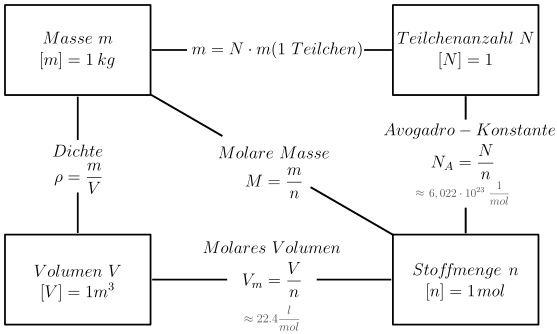
\includegraphics[width = 69mm]{Bilder/Zusammenhang.png}\\
\begin{enumerate}[noitemsep]
    \item \textbf{Energie:} $1eV=1.602\cdot 10^{-19}J$,    $1cal=4.18J$
    \item \textbf{Druck:} $1$Pa=$9.892$atm=$1.0\cdot 10^{-5}$bar=$7.5\cdot 10^{-3}$torr
    \item \textbf{Stoffmenge: } $1$mol = $6.022\cdot 10^{23}$ Teilchen (Avogadrokonst.)
    \item \textbf{Länge:} $1\text{Å}=10^{-10}m$
    \item \textbf{Standardbedingungen Thermodynamik: } $25C=298K$,  $1$bar,  $1$mol, $1$ cal
    \item \textbf{Standardbedingungen Elektrochemie: } $25C=298K$,  $1$atm, Konzentration $1$M
\end{enumerate}
}


\subsection{1.2 Allgemeines}{

    \begin{itemize}[noitemsep, leftmargin=*]
        \item \textbf{Kinetische Energie:} $E_{kin} = \frac{1}{2} \cdot m \cdot v^2$
        \item \textbf{Potentielle Energie:} $E_{pot} = m \cdot g \cdot \Delta h$
        \item \textbf{Elektrostatische WW:} $E_{el}=\frac{\kappa Q_1Q_2}{d^3}$\quad $\kappa = \frac{1}{4\pi \epsilon_0}$
        \item \textbf{Photonenenergie: } $E_\gamma = h\cdot f = \frac{h\cdot c}{\lambda}$
        \item \textbf{de-Broglie-Wellenlänge: } $\lambda = \frac{h}{m\cdot v}$
        \item \textbf{spez. wärmekapazität: }$C_s=\frac{q}{m\cdot\Delta T}$
    \end{itemize}
}


\subsection{1.3 Trends im Periodensystem}{
\begin{itemize}[noitemsep, leftmargin=*]
    \item \textbf{Ionisierungsenergie: }Energie, die nötig ist, um ein Elektron aus der neutral geladenen Atom zu entfernen.
    \item \textbf{Elektronenaffinität:} Frei werdende Energie, wenn ein neutrales Atom ein Elektron aufnimmt.
    \item \textbf{Elektronegativität:} Die Elektronegativität ist ein Maß für das Bestreben eines Atoms, innerhalb eines Moleküls von benachbarten Atomen die Elektronen anzuziehen.

    
\end{itemize}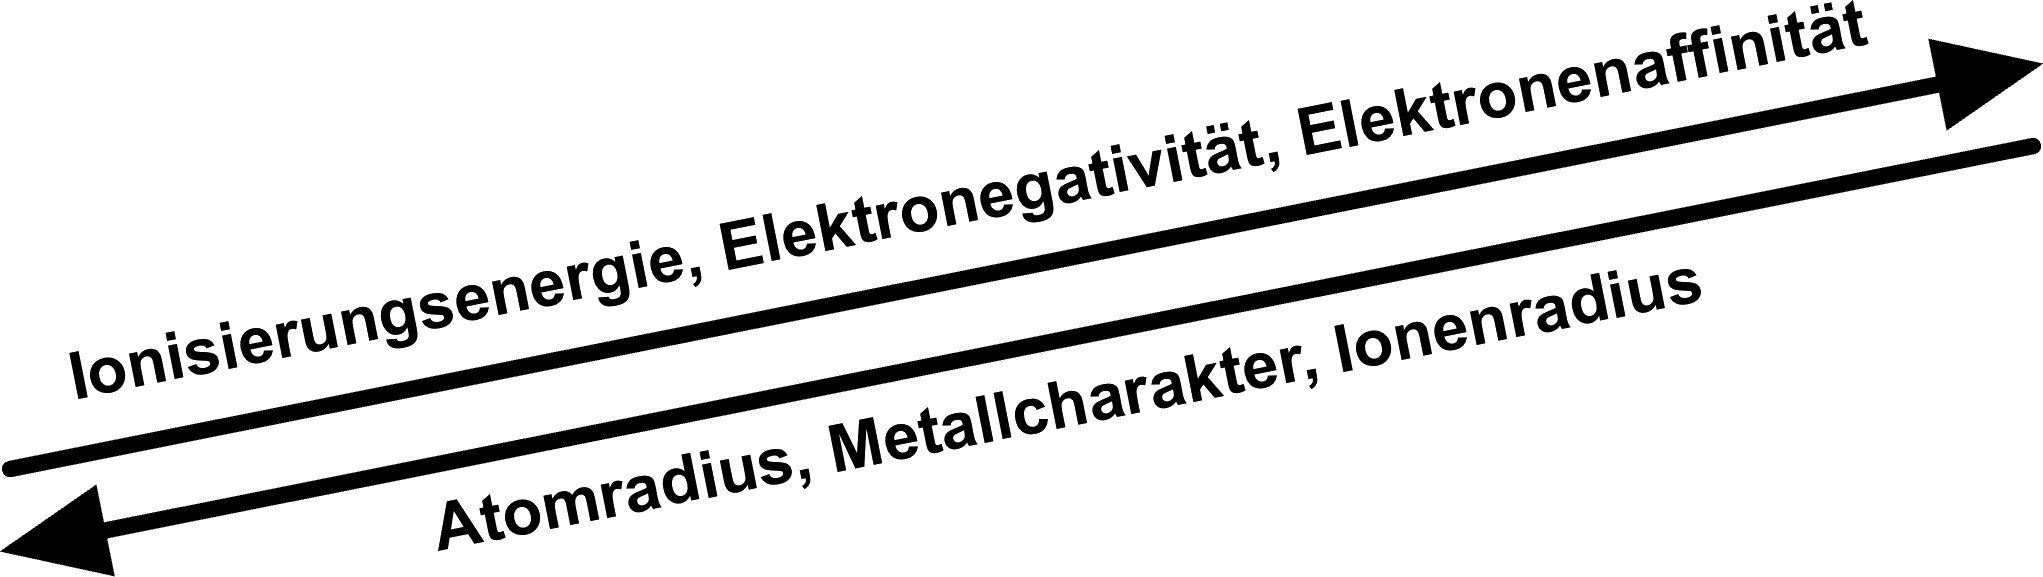
\includegraphics[width = 68mm]{Bilder/TrendsimPSE.png}
}

\section{2. Atome}
\subsection{2.1 Quantenmechanik}{
    \begin{itemize}[noitemsep, leftmargin=*]
        \item Ordnungszahl = \#Protonen = \#Elektronen 
        \item Massenzahl = Anzahl Protonen + Anzahl Neutronen
    \end{itemize}
    Elektronen haben Teilchen und Welleneigenschaften. Daraus folgt, dass sich Energie und Position eines Elektrons nicht mit der gleichen Genauigkeit bestimmen lassen (Heisenberg'sche Unschärferelation).\\
    \textbf{Effektive Kernladung:}   $Z_{eff} = Z-S$\\
    $Z$ = Anzahl Protonen, $S$ = Anzahl $e^-$ auf innere Bahnen
    \vspace{1mm}\\
    Innerhalb einer Periode nimmt effektive Kernladung von links nach rechts zu. Daraus folgt, dass   stärker an den Kern gebunden sind, der Atomradius nimmt ab. 
}


\subsection{2.2 Orbitale}{
    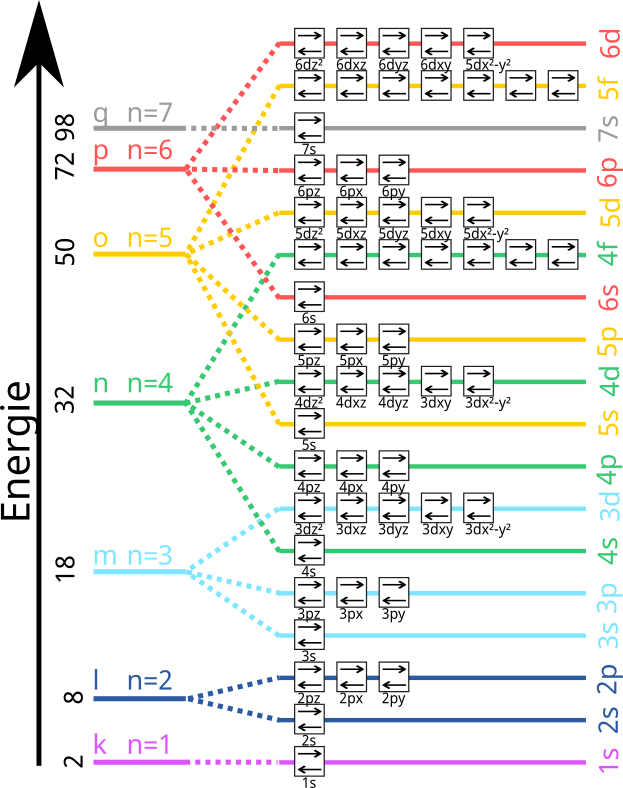
\includegraphics[width = 5cm, angle=-90]{Bilder/Energieniveau.png}
    \begin{itemize}[noitemsep, leftmargin=*]
        \item Orbitale mit dem gleichen n-Wert heissen Schalen. 
        \item Orbitale mit dem selben n- und l-Werten heissen Unterschalen.
        \item Jede Schale mit Quantenzahl n hat n Unterschalen.
        \item Die Drehimpulszahl bestimmt die Form der Orbitale.
        \item Jede Unterschale hat $2l + 1$ Orbitale.
    \end{itemize}
    \textbf{Hauptquantenzahl $n$:} Je grösser n, desto weiter ist das elektron vom Kern entfernt. $n \in [1, 2, 3, 4]$. n bedingt $l$ \& $m$
    \vspace{1mm}\\
    \textbf{Drehimpulsquantenzahl $l$:} Bestimmt Form der Orbitale. $l \in [0, n-1]$
    \vspace{1mm}\\
    \textbf{Magnetische Quantenzahl $m_l$:} Beschreibt  Orientierung des Orbitals im Raum $m_l \in [-l, l]$
    \vspace{1mm}\\
    \textbf{Spinnquantenzahl $m_s$:} Zu verstehen als Drehimpuls. Spin up $\uparrow$, Spin-down $\downarrow$ 
    \begin{itemize}[noitemsep, leftmargin=*]
        \item s-Orbital $\rightarrow$ Kugelförmig.
        \item p-Orbital $\rightarrow$ Hantelförmig.
        \item d-Orbital $\rightarrow$ Meistens Vierblättriges Kleeblatt.
    \end{itemize}
    \textbf{Pauli-Prinzip:} Jedes Orbital kann von maximal zwei Elektronen besetzt werden (Eins mit Spin-up, eins mit Spin-down).
    \vspace{1mm}\\
    \textbf{Hund'sche Regel:} Möglichst viele Elektronen haben den gleichen Spin,  weswegen es energetisch günstiger ist, wenn alle 
    Orbitale der äussersten Schale gefüllt werden, als wenn die Hälfte dieser Orbitale ganz gefüllt werden.\par
    \vspace{1mm}\centering
    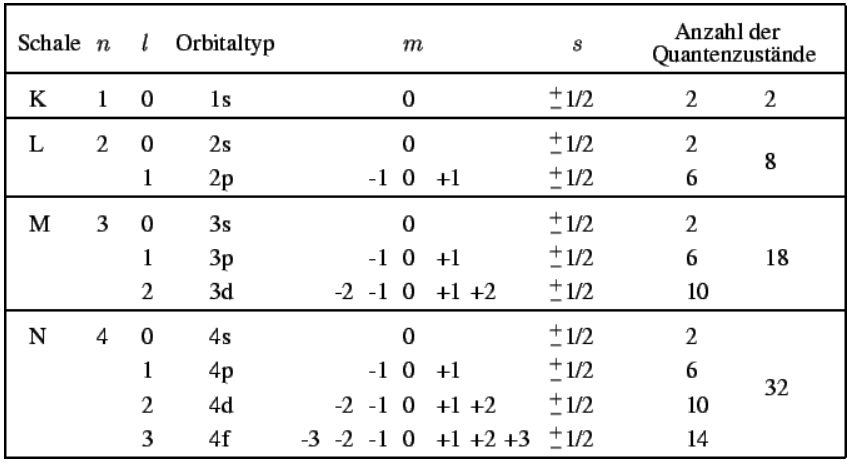
\includegraphics[width=54mm]{Bilder/Quantenzahlen.PNG}
    }


	
\section{3. Chemische Bindungstypen}

\subsection{3.1 Kovalente Bindungen}{
    Zwei Atome teilen sich ein Elektronenpaar. Bsp.:\\
    


    \textbf{Oktettregel:} \#Bindungen =8-\#VE\\
    Nur für Elemente der 1. \& 2. Hauptgruppe gilt Oktettregel strikt. 
    Ab dritten HG können Elemente auch mehr Bindungen eingehen.\\
    \textbf{!}Bei H und He $\rightarrow$ \#Bindungen = 2 - \#VE
}


\subsection{3.2 Polarität \& Dipolmoment}{
    \begin{itemize}[noitemsep, leftmargin=*]
    \item $\Delta EN<0.5$: Gleichmässige Verteilung der Elektronen zwischen Atomen, kein Dipolmoment.
    \item $\Delta EN>0.5$: Polare Bindung, $e^-$ näher beim elektronegativen Atom ($\delta^-$).
    Ungleichmässige Verteilung der Elektronen $\rightarrow$ Dipolmoment.
    
    \end{itemize}
}

\subsection{3.3 Formalladung}{
    Wenn ein Atom mehr/weniger Bindungen macht, als nötig sind um ein VE-Oktett zu erreichen, resultiert eine Formalladung auf den Atom.\\
    \textbf{Bestimmung der Formalladung:}
    \begin{enumerate}[noitemsep,leftmargin=*]
        \item Alle Bindungen im Molekül spalten (gleichmässige Aufteilung zwischen Bindungspartnern.)
        \item Formalladung je Atom = $\# VE- \# e^-$(nach Spaltung)
        \item Formalladungen aufsummieren $\rightarrow$ effektive Ladung des Moleküls.
        \item \textbf{Homolytische Spaltung:} Bindung gleichmässig in der Mitte trennen\\
        \vspace{1mm}

    \end{enumerate}
}


\subsection{3.4 Bindungslänge \& Bindungsstärke}{
    \textbf{Länge:} Dreifach $<$ Doppelt $<$ Einfach\\
    \textbf{Stärke:} Dreifach $>$ Doppelt $>$ Einfach\\
    \textbf{Ein Molekül ist am stabilsten, wenn:}
    \begin{itemize}[noitemsep, leftmargin=*]
    \item am wenigsten Formalladungen.\item Formalladung nicht zu vermeiden sind, wenn geringste Ladungstrennung auftritt.\item negative (positive) Formalladungen auf elektronegativen (-positiven) Atomen.
    \end{itemize}
}


\subsection{3.5 Ionische Bindung}{
    Ein Atom gibt einem anderen Atom Elektronen ab $\rightarrow$ Kationen(+) und Anionen(-) entstehen. Bindung durch elektrostatische Anziehung. Ionische Bindung erst ab $\Delta EN > 1.7$\\
    Atom mit niedrigerer EN gibt Elektron ab $\leftrightarrow $.\\
    Die freiwerdende Energie, wenn sich Anion \& Kation im Gitter anordnen nennt man : $\Delta H_{Gitter}$
}


\subsection{3.6 Metallische Bindung}{    

        \begin{minipage}{25mm}
            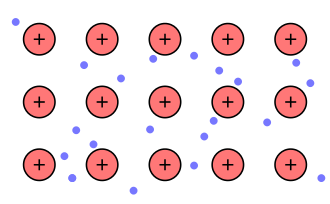
\includegraphics[width=2.5cm]{Bilder/Metallische Bindung.png}
        \end{minipage}
        \begin{minipage}{42mm}
            Positiv geladene Kerne umgeben von einer negativ geladenen Elektronenwolke. Metalle haben
            Defizit an VE $\rightarrow$ zu wenig VE, um Kovalente Bindung einzugehen. Frei bewegliche Ladungen 
            (Elektronenwolke) sind Ursache für gute Strom- und Wärmeleitfähigkeit.
        \end{minipage}
}


\section{4. Molekülmodelle}
\subsection{4.1 VSEPR}{

\textbf{Bestimmung des Modells:}
\begin{enumerate}[noitemsep,leftmargin=*]
    \item Zentralatom des Moleküls bestimmt.
    \item Anzahl Liganden Bestimmen
    \item Bestimmung der freien Elektronenpaare $\rightarrow$ Tabelle
\end{enumerate}

\textbf{Bindungsordnung (BO)}=  $0,5\cdot$(\# $e^-$in bindenden MO $-$ \# $e^-$ in anti-bindenden MO)\\
Je höher BO, desto stabiler das System, stärker die Bindung und kürzer die Bindung.
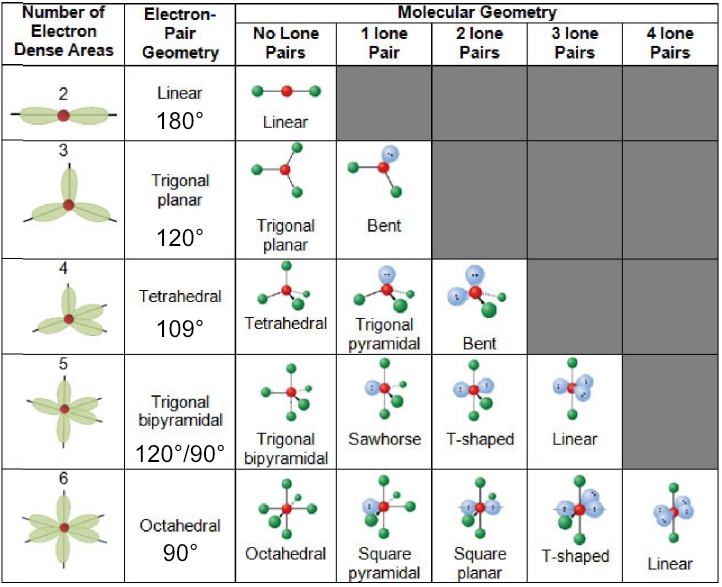
\includegraphics[width=68mm]{Bilder/VSEPER.PNG}
}


\subsection{4.2 Molekül-Orbital-Modell}{
    Bindung entsteht durch das Überlappen der Atomorbitale zweier
    Atome wodurch zwei neue Molekülorbitale gebildet werden.\\
    \begin{minipage}{35mm}
        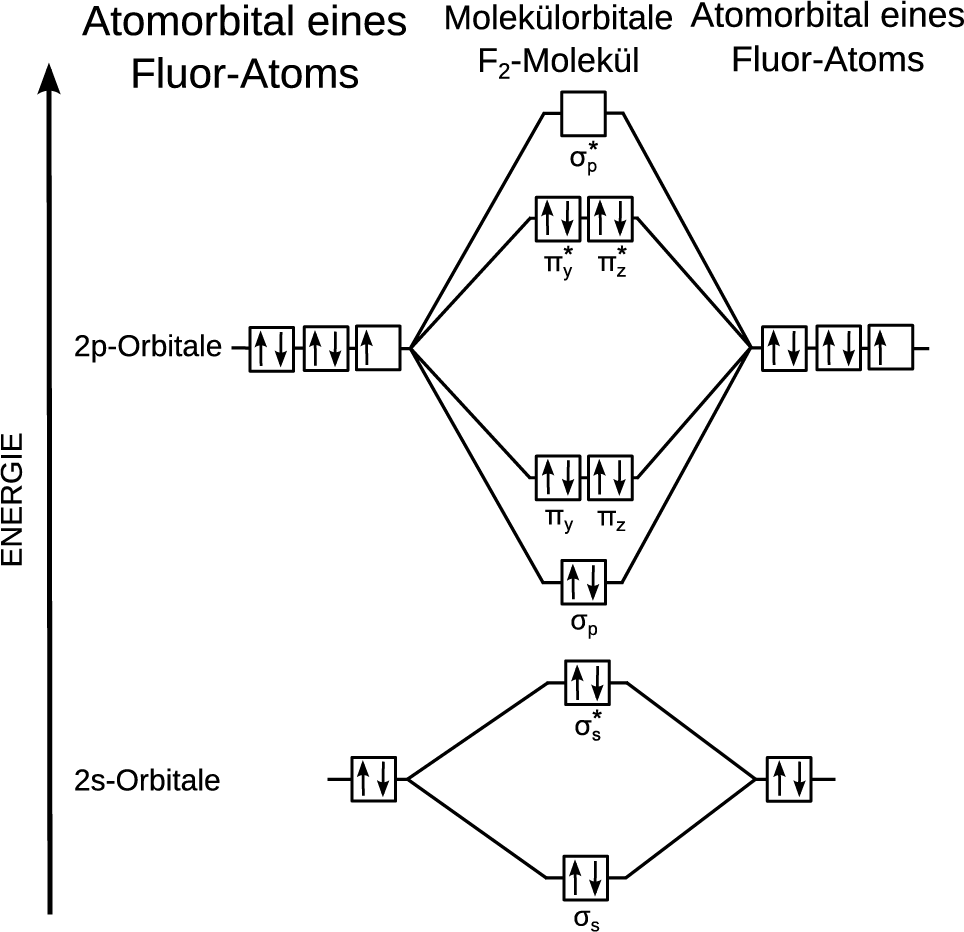
\includegraphics[width=3.5cm]{Bilder/Molekuelorbitalmodell.png}
    \end{minipage}
    \begin{minipage}{32mm}
        \textbf{$\sigma$-Bindung:} Atomorbitale überlappen entlang der internuklearen Achse.\\
        \textbf{$\pi$-Bindung:} Atomorbitale überlappen parallel zur internuklearen Achse.\\
        Diagramm von unten nach oben auffüllen. Mit * markierte Orbitale sind antibindend.
    \end{minipage}
    \textbf{Ferromagnetische Eigenschaften von Molekülen:}\\
    \textbf{Paramagnetisch: }Das Molekül hat ungepaarte Elektronen und wird daher
    von einem Magnetfeld angezogen.\\
    \textbf{Diamagnetisch: }Das Molekül hat keine ungepaarten Elektronen und wird
    daher von einem Magnetfeld leicht abgestossen.\\
    1 Pfeil in Box $\rightarrow$ Paramagnetisch, sonst Diamagnetisch
}

\subsection{4.3 Hybridisierung}{
Verschmelzen von verschiedenen Orbitalen in einem Molekül.
    \begin{itemize}[noitemsep, leftmargin=*]
    \item Bei der sp-Hybridisierung verschmelzen ein s- und ein p-Orbital miteinander. Bsp.: ethin (HC$\equiv$CH)
    \item Bei der $sp^2$-Hybridisierung kommt zu einer Hybridisierung eines s-Orbitals und zwei p-Orbitalen. Bsp.: Ethen (H2C=CH2)
    \item Bei der $sp^3$-Hybridisierung verbindet sich ein kugelförmiges s- und drei hantelförmige p-Orbitale. Bsp.: Methan(CH4)
\end{itemize}
\centering
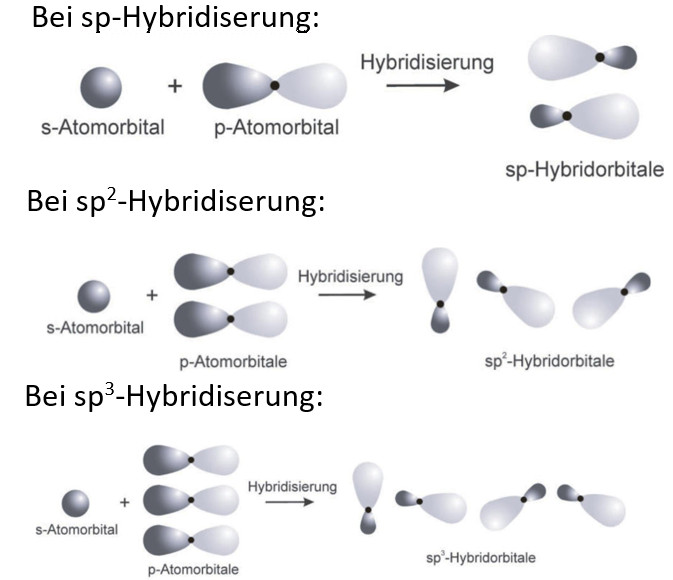
\includegraphics[width=60mm]{Bilder/Hybridorbitale.png}



}



\section{5. Aggregatszustände}

\subsection{5.1 Intermolekulare Wechselwirkungen}{
\begin{enumerate}[noitemsep,leftmargin=*]
    \item \textbf{Wasserstoffbrücken} (stark)\\
     Entstehen zwischen \ce{H} und \ce{O,N,F} Atomen
    \item \textbf{Dipol-Dipol-Wechselwirkungen} (mittel) \\
     Entstehen durch polare Bindungen ($\Delta EN>0.5$)
    \item \textbf{Van-der-Waals-WW/Dispersionskräfte} (schwach)\\
     Entstehen durch temporäre Fluktuationen der Elektronen $\rightarrow$ temporärer Dipol,
     \textbf{Gibts es immer}.Grosse und lange Moleküle haben die stärksten Dispersionskräfte.
\end{enumerate}
}

\subsection{5.2 Flüssigkeiten}{
    \textbf{Gefrierpunktserniedrigung: } $\Delta T_f=K_fm$\\
    $K_f=$ Kryoskopische Konst.     $m=$ Molalität $\left[\frac{mol}{kg}\right]$\\
    Je tiefer die \textbf{Viskosität}, desto grösser die Mobilität der Moleküle. Viskosität proportional
    zur Stärke der WW. Je höher die Viskosität, desto dickflüssiger. 
}

\cb
\subsection{5.3 Ideale Gase}{
    \begin{itemize}[noitemsep, leftmargin=*]
        \item Wir machen 2 Annahmen:
        \begin{itemize}[noitemsep, leftmargin=*]
            \item Gasteilchen wechselwirken nicht.
            \item Gasteilchen haben kein Volumen.
        \end{itemize}
        \item Ideales Gasgesetz: $pV = nRT=N kT$
        \item Dichte $\rho = M\frac{n}{V}=M\frac{p}{RT}$
        \item R ist die universelle Gaskonstante.\vspace*{1mm}
        \item Quadr. Mittelwert der Geschwindigkeit der Gasmoleküle:\\ $u_{rms}=\sqrt{3RT/M}$
        \item $M\left[ gmol^{-1} \right]$, $d\left[ gL^{-1} \right], V\left[L\right]$
    \end{itemize}
    \vspace{1mm}
    Bei hohen Drücken verhalten sich Gase nicht mehr ideal $\rightarrow$  korrigierte
    ideale Gasgleichung:\\\quad\quad$(p+\frac{n^2A}{V^2})(V-nb)=nRT$\\
\textbf{Partialdruck:} Der Partialdruck ist der Anteil eines Gases am Druck des betrachteten Gasgemisches. Partialdrücke einer Gasmischung sind immer kleiner als der Gesamtdruck.\vspace{0.5mm}\\
$p_i=n_i\cdot\frac{RT}{V}$ Gesamtdruck $=\Sigma$ aller Partialdrücke
}


\subsection{5.4 Osmotischer Druck}{
    Der Druck der benötigt würde, um Fluss von Lösungsmittelteilchen zu unterdrücken heisst
osmotischer Druck.
\begin{equation*}
    \Pi = \left(\frac{n}{V}\right)RT=MRT \text{\quad} M = \text{Molarität}
\end{equation*}
}





\section{6. Thermodynamik}
\subsection{6.2 0. Haupsatz}{
\begin{itemize}[noitemsep, leftmargin=*]
    \item Sind 2 Systeme wärmeleitend verbunden, dann haben beide Systeme die gleiche
            Temperatur.\textbf{Thermisches Gleichgewicht.}
    \item Wenn drittes System mit den anderen Systemen wärmeleitend verbunden ist $\rightarrow$ 
         drittes System hat gleiche Temperatur.
\end{itemize}

}
\subsection{6.2 1. Haupsatz}{
\begin{itemize}[noitemsep, leftmargin=*]
    \item Energie kann weder aus dem Nichts erzeugt werden, noch kann sie vernichtet werden \textbf{Energieerhaltung}.
    \item Energie kann von einem System nur mit der Umgebung mittels Wärme oder Arbeit ausgetauscht werden.
    \item Der 1. Hauptsatz der Thermodynamik verbindet die innere Energie eines Systems mit der am System/vom System verrichteten Arbeit und der aufgenommenen/abgegebenen Wärme:\\
    $\Delta U = \Delta W+\Delta Q$\\
    $\Delta E < 0 \rightarrow \text{exergon}$,   $\Delta E > 0 \rightarrow \text{endergon}$\\
    $Q=$Wärme   $W=$Arbeit   $U=$Innere Energie (manchemal E)
\end{itemize}
}

\subsection{6.3 2. Hauptsatz}{
\textbf{Entropie:} Mass an Unordnung. Ist eine Zustandsfunktion
\begin{itemize}[noitemsep, leftmargin=*]
    \item irreversibler Prozess:  $\Delta S > 0$, reversibler Prozess $\Delta S = 0$
    \item Die Entropie nimmt immer zu.
\end{itemize}
\begin{equation*}
    \Delta S = \frac{q_{rev}}{T}=S_{Ende}-S_{Anfang}\\
\end{equation*}
\begin{equation*}
    \Delta S = nR\cdot \ln\left(\frac{V_{Ende}}{V_{Anfang}}\right)
\end{equation*}
\quad $q_{rev}=$ Wärmemenge bei reversiblem Prozess
}

\subsection{6.5 Gibbs Energie $\Delta G$}{
    $\Delta G = \Delta H -T\cdot\Delta S$ \\
    $\Delta G_{rxn} = \Delta G_{Produkte} - \Delta G_{Edukte}$\\
    $\Delta {G^o_f} = 0$ für Elemente
    \begin{itemize}[noitemsep, leftmargin=*]
        \item \textbf{Spontan:} $\Delta G < 0$,  
        \textbf{Nicht spontan:} $\Delta G > 0$
    \end{itemize}
    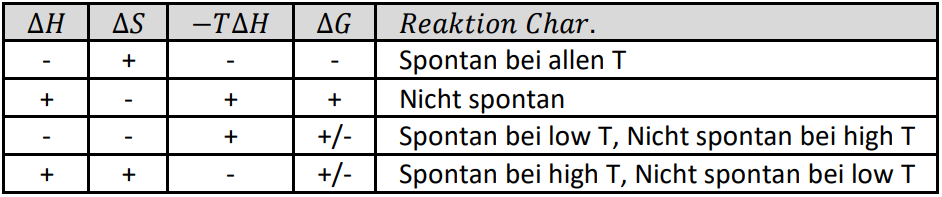
\includegraphics[width=68mm]{Bilder/Gibs.png}
}

\subsection{6.4 Enthalpie$\Delta H$}{
Bei konstantem Druck aufgenommenen/ abgegebenen Wärmemenge\\
$\Delta H = \Delta E + p\Delta V = (q_p+w)-w=q_p$
\begin{enumerate}[noitemsep,leftmargin=*]
    \item Endotherm: $\Delta H > 0$ (System nimmt Wärme auf)
    \item Exotherm: $\Delta H < 0$ (System gibt Wärme ab)
\end{enumerate}

\textbf{Reaktionsenthalpie:}\\ 
    $\Delta H = \Delta H_{Produkte} - \Delta_{Edukte}$\vspace{1mm}\\
\textbf{Bildungsenthalpie:} \\
    $\Delta H_f = \sum n\cdot H_f(Produkte) - \sum m\cdot H_f(Edukte)$\\
    $n,m = $ Anzahl Moleküle\\
Falls Edukt/Produkt nur 1 Element $\rightarrow H_f=0$\\

    \textbf{Intensive Zustandsgrößen: }Druck, absolute Temperatur\\
    \textbf{Extensive Zustandsgrößen: }Volumen, Stoffmenge, Entropie\\
    \textbf{Thermodynamische Potentiale (Zustandsgröße): }innere Energie, freie Energie, Enthalpie, Gibbs-Energie\\
    \textbf{Prozessgrößen: }Wärme, Arbeit

\textbf{Satz von Hess:} $\Delta H_{rxn}=\Delta H_1 + \Delta H_2 + \dots + \Delta H_n$
}





\section{7. Kinetik}
\subsection{7.1 Reaktionsgeschwindigkeit}{
    $-aV-bB-(\dots)+cC+dD+(\dots)=0$

    \begin{equation}\label{eq:1}
        \textbf{Reaktionsgesetz: }r=\frac{1}{\nu}\frac{d\left[X_i\right]}{dt}=k\prod_{i=1}{\left[N_i\right]}^{|\nu_i|}
    \end{equation}\\
    $\nu=$ Stöchiometrischer Koeffizient, für Edukte \textbf{+} für Produkte \textbf{-}
    $k=A\cdot\exp\left(-\frac{E_a}{RT}\right)$ $A$=Frequenzfak., $E_a$=Aktivierungsenergie, 
    $k=$ Geschwindigkeitskoeffizient. \\

\textbf{Bestimmung der reaktionsgeschwindigkeit an Bildungsgeschwindigkeit}\\
\begin{enumerate}[noitemsep,leftmargin=*]
    \vspace*{-4.5mm}
    \item Schauen, von welchem Molekül Geschwindigkeit gefragt, von welchem gegeben
    \item Koeffizienten der betroffenen Moleküle merken
    \item In \ref{eq:1} einsetzen und nach gesuchter Geschwindigkeit auflösen
\end{enumerate}
}

\subsection{7.2 Reaktionsordnung}{
Reaktionsordnung bezüglich eines Edukts = Betrag seines stöch. Koeffizienten.
Gesamtordnung = Summe aller Ordnungen der Edukte.\vspace*{1mm}


Bsp.. \ce{NH_4^+} + \ce{NO_2^-} $\longrightarrow $ \ce{N_2} + \ce{2H_2O} mit\\
 $\textbf{Geschwindigkeitsgesetz: }r=k{\left[\ce{NH_4^+}\right]}^1{\left[\ce{NO_2^-}\right]}^1$\\

    $m_{NH_4^+}=1; \quad
    m_{NO_2^-}=1; \quad
    m_{N_2}=0 ;\quad
    m_{H_2O}=0$\\

    Gesamtordnung der Reaktion ist: $m_{tot}=\sum m_i=2$
    \begin{itemize}[noitemsep,leftmargin=*]
        \item \textbf{0. Ordnung: } konzentrationsunabhängig
        \item \textbf{1. Ordnung: } Abhängig von Konzentration 1 Reaktanten
        \item \textbf{2. Ordnung: } Abhängig von Konzentration 2 Reaktanten
    \end{itemize}
    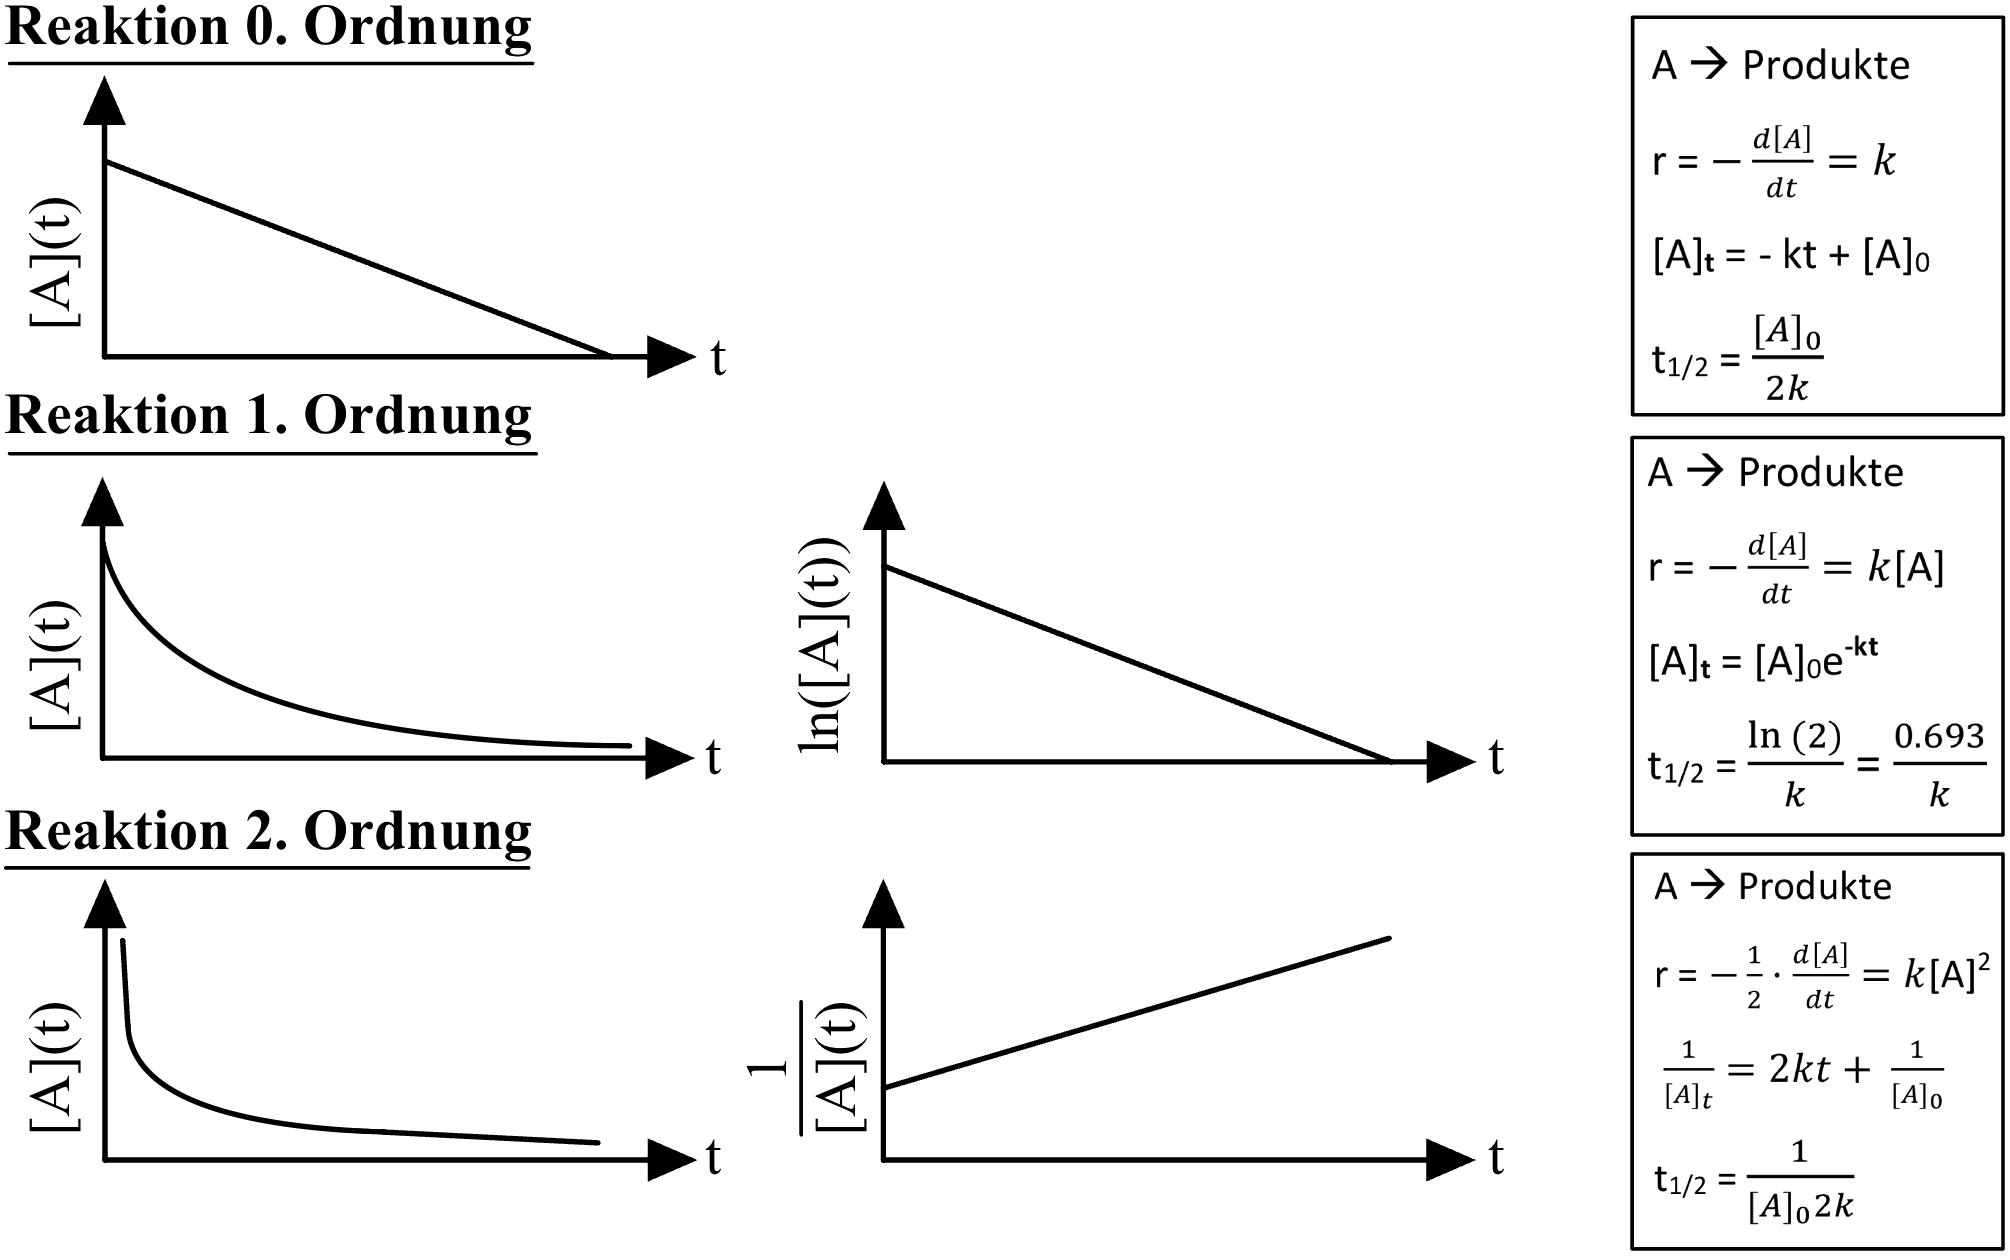
\includegraphics[width=69mm]{Bilder/Reaktionsordnung2.png}
    
}
\cb
\subsection{7.3 Molekularität einer Reaktion}{
    Anzahl der an Elementarreaktionen teilnehmenden Molekülen.\\
    \textbf{Elementarreaktion:} Einzelner, irreversibel Schritt.\\
    Unimolekular: A $\longrightarrow $ Produkten\\
    Bimolekular: A + B $\longrightarrow $ Produkten\\
    Trimolekular: 2A + B $\longrightarrow $ Produkten\\
    \textbf{Mehrstufige reaktion: }Reaktion aus mehreren Elementarreaktion Bsp.:\\
    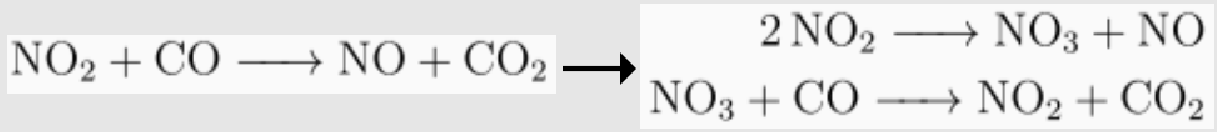
\includegraphics[width=68mm]{Bilder/Mehrstufigereaktion.PNG}
    \textbf{Geschwindigkeitsgebender Schritt: }Einzelne Elementarreaktionen oftmals nicht gleich schnell
    $\rightarrow$ Geschwindigkeit annäherbar durch Geschwindigkeit des langsamsten Schritts.\\
    \textbf{Reaktions und Geschwindigkeitsgesetz bestimmen:}

    \begin{enumerate}[noitemsep,leftmargin=*]
        \item Alle Gleichungen addieren, Gleiches kürzen $\rightarrow$ Reaktion
        \item Produkte langsamster reaktion $\rightarrow$ Geschwindigkeitsgesetz
    \end{enumerate}

    \begin{itemize}[noitemsep,leftmargin=*]
        \item \textbf{Qualitative Temperaturabhängigkeit von k:}\\
        Die Erhöhung der Temperatur um $10^oC$ hat eine Verdoppelung der reaktionsgeschwindigkeit $r$
        bzw. des Geschwindigkeitskoeffizient $k$ zur Folge.
        \item \textbf{Qualitative Temperaturabhängigkeit von k:}\\
        \vspace{1mm}
        $k(T)=A\cdot\exp (-\frac{E_a}{RT})\quad\ln (k(T))=-\frac{E_a}{RT}+\ln (A)$
    \end{itemize}
}
\section{8. Säure und Basen}
\subsection{Allgemein}{
    Für die Reaktion $aA+bB\leftrightarrows cC+dD$
    \begin{equation*}
        K=\frac{k\_Hin}{k\_R\ddot{u} ck}=\frac{\left[Produkte\right]}{\left[Edukte\right]}=\frac{{\left[C\right]}^c{\left[D\right]}^d}{{\left[A\right]}^a{\left[B\right]}^b}
    \end{equation*}
    $K\gg 1\rightarrow \text{GGW rechts} $\quad $K\ll 1\rightarrow \text{GGW links}$
    }

    
\subsection{8.1 Prinzip von le Châtélier}{
    \begin{itemize}[noitemsep,leftmargin=*]
        \item \textbf{Konzentrationsänderung}: Erhöhung der Reaktanten führt zu Beschleunigung der Hin-Reaktion
        \item \textbf{Druckänderung}: Wird Druck in System erhöht $\rightarrow$ GGW verschiebt sich in Richtung Seite mit weniger teilchen.
        \item \textbf{Temperaturänderung}: Endotherme Reaktion wird bei Erhöhung bevorzugt.
    \end{itemize}
}


\subsection{8.2 Brönsted-Definition}{
    \begin{minipage}{34mm}
        S-B-Reaktion sind GGW-Reaktionen.
        \begin{itemize}[noitemsep,leftmargin=*]
        \item Säuren geben $H^+$ ab \\(Protonendonatoren).
        \item Basen nehmen $H^+$ auf \\(Protonenakzeptoren).
        \item Schwache Säure: $K\ll1$\\ GGW bei $HA$
        \item Starke Säure: $K\gg1$\\GGW bei $A^-$
    \end{itemize}
    \end{minipage}
    \begin{minipage}{34mm}
        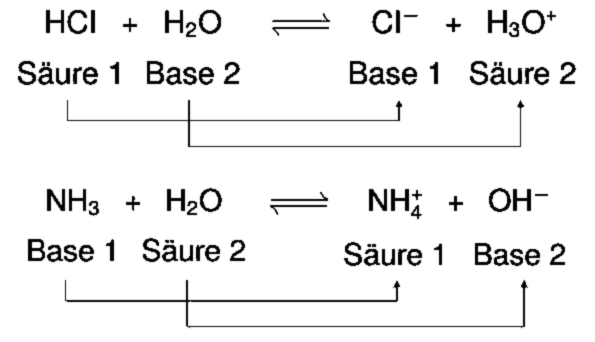
\includegraphics[width=34mm]{Bilder/SaureBaseReaktion.png}
        \vspace*{1mm}
        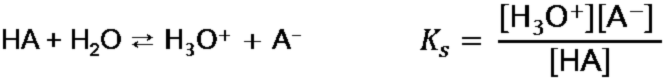
\includegraphics[width=34mm]{Bilder/SaureBaseReaktion2.png}
    \end{minipage}
    $pH=-\lg (\left[H_3O^+\right]),\; pOH=-\lg(\left[OH^-\right])\\14=pOH+pH$
}


\subsection{8.3 PH-Skala $pK_S=-\log K_S$}{ 
    \begin{minipage}{35mm}
        \begin{itemize}[noitemsep,leftmargin=*]
            \item Saure Lsg. pH-Wert $<7$
            \item Basische Lsg. pH-Wert $>7$
    \end{itemize} 
        \end{minipage}
    \begin{minipage}{35mm}
        \begin{itemize}[noitemsep,leftmargin=*]
            \item hoher $K_S\rightarrow$ starke Säure
            \item tiefer $K_S\rightarrow$ starke Base
        \end{itemize}
\end{minipage}
\textbf{pH-Wert bestimmen:} $pH=-\log(c(\left[S\ddot{a}ure \right]))=14-pOH$
}


\section{8.4 Redoxreaktion}
\subsection{Allgemeines}{
    \begin{itemize}[noitemsep,leftmargin=*]
        \item Reaktion bei welcher Elektronen zwischen reaktionspartnern ausgetausch werden
        \item \textbf{Oxidation:} Abgabe von $e^-$, Oxidationszahl wird erhöht (Reduktionsmittel wird oxidiert).
        \item \textbf{Reduktion:} Annahme von $e^-$, Oxidationszahl wird gesenkt (Oxidationsmittel wird reduziert).
    \end{itemize}
    \textbf{Oxidationszahl:}$\triangleq$\# VE eines Atoms-\#Elektronen verbleibend am 
    Atom nach \textbf{heterolytischer Spaltung:}\par
    \centering
    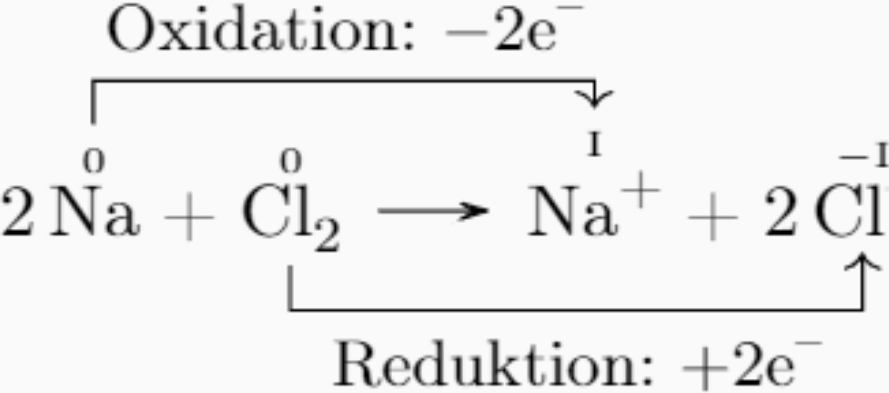
\includegraphics[height=16mm]{Bilder/Redox.PNG} 
    }


\subsection{8.5 Heterolytische Spaltung}{
    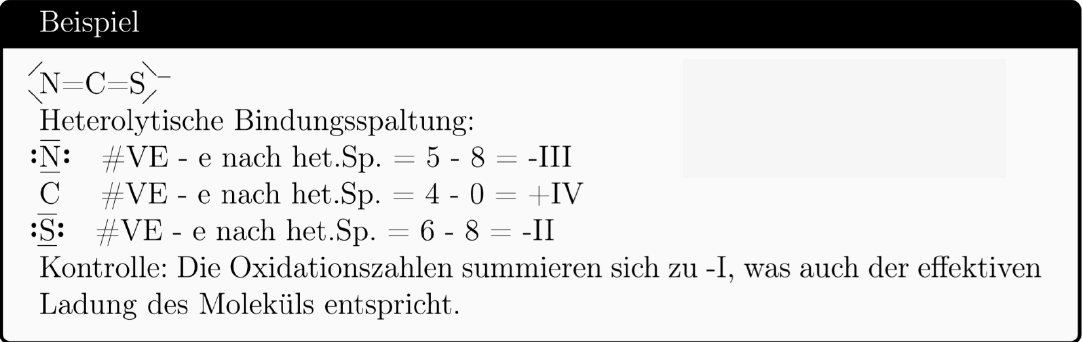
\includegraphics[width=68mm]{Bilder/HeterolytischeSpaltung.PNG}
    \begin{enumerate}[noitemsep,leftmargin=*]
        \item Gesamtladung = Summe der Oxidationszahlen.
        \item Homonukleare Moleküle An haben die Oxidationszahl
        \item Bei einatimigen Ionen: Ladung = Oxidationszahl.
        \item Wasserstoff am Metall → Hydrid (-I)
        \item Wasserstoff am Nichtmetall → Proton (+I)
        \item Sauerstoff oft –II
        \item Fluor immer –I, da elektronegativestes Element
    \end{enumerate}
    \textbf{Oxidationsmittel:} Stoff, welcher andere Stoffe oxidiert und dabei selbst reduziert wird, da er gerne Elektronen aufnimmt.
    \textbf{Reduktionsmittel:} Stoff, welcher andere Stoffe reduziert und dabei selbst oxidiert wird, da er gerne Elektronen abgibt.
}
\subsection{8.6 Galvanische Zelle}{
\begin{minipage} {35mm}
    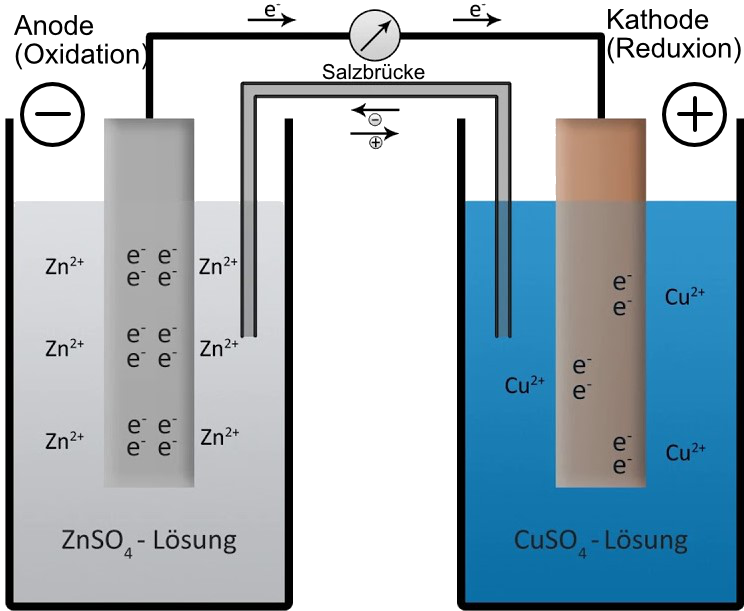
\includegraphics[width=35mm]{Bilder/GalvanischeZelle.png}
\end{minipage}
\begin{minipage}{33mm}
    $e$ fliessen von der Anode zur Kathode. Anode gibt $e$ ab. Kathode nimmt $e$ auf.
    Oxidation an Anode. Reduktion an Kathode.\\ 
    Überschüssige Sulfationen wandern über salzbrücke zurück $\rightarrow$ Ladungsausgleich.
\end{minipage}


\vspace{1mm}Die Zellspannung $E_{zelle}$ gibt Unterschied zwischen den Elektrodenpotentialen wieder. Der Unterschied in diesem Potential ist die EMK. Zellspannung in  Volt.
$E_{Zelle}=E_{Red}(Kat.)-E_{Red}(Ano.)=E_{Red}(Red)-E_{Red}(Ox)$
}
\mbox{}
\end{multicols*} 
\end{document}